%%
% ximera activiteit
% Copyrigth
%
\documentclass{ximera}
%
% Opties (enkel te gebruiken voor lokale testen; NOOIT committen met opties)
%
%\pdfOnly{\providecommand\showtodonotes{}}
%\newcommand\xmnouitweiding{}


%
% copied from https://github.com/mooculus/calculus
%
\usepackage[utf8]{inputenc}


\graphicspath{
	{./}
	{goniometrie/}
}


%\usepackage{todonotes}
%\usepackage{mathtools} %% Required for wide table Curl and Greens
%\usepackage{cuted} %% Required for wide table Curl and Greens
\newcommand{\todo}{}

% Font niet (correct?) geinstalleerd in MikTeX?
%\usepackage{esint} % for \oiint
%\ifxake%%https://math.meta.stackexchange.com/questions/9973/how-do-you-render-a-closed-surface-double-integral
%\renewcommand{\oiint}{{\large\bigcirc}\kern-1.56em\iint}
%\fi


\newcommand{\mooculus}{\textsf{\textbf{MOOC}\textnormal{\textsf{ULUS}}}}

\usepackage{tkz-euclide}\usepackage{tikz}
\usepackage{tikz-cd}
\usetikzlibrary{arrows}
\tikzset{>=stealth,commutative diagrams/.cd,
  arrow style=tikz,diagrams={>=stealth}} %% cool arrow head
\tikzset{shorten <>/.style={ shorten >=#1, shorten <=#1 } } %% allows shorter vectors

\usetikzlibrary{backgrounds} %% for boxes around graphs
\usetikzlibrary{shapes,positioning}  %% Clouds and stars
\usetikzlibrary{matrix} %% for matrix
\usepgfplotslibrary{polar} %% for polar plots
\usepgfplotslibrary{fillbetween} %% to shade area between curves in TikZ
\usetkzobj{all}
\usepackage[makeroom]{cancel} %% for strike outs
%\usepackage{mathtools} %% for pretty underbrace % Breaks Ximera
%\usepackage{multicol}
\usepackage{pgffor} %% required for integral for loops



%% http://tex.stackexchange.com/questions/66490/drawing-a-tikz-arc-specifying-the-center
%% Draws beach ball
\tikzset{pics/carc/.style args={#1:#2:#3}{code={\draw[pic actions] (#1:#3) arc(#1:#2:#3);}}}



\usepackage{array}
\setlength{\extrarowheight}{+.1cm}
\newdimen\digitwidth
\settowidth\digitwidth{9}
\def\divrule#1#2{
\noalign{\moveright#1\digitwidth
\vbox{\hrule width#2\digitwidth}}}





\newcommand{\RR}{\mathbb R}
\newcommand{\R}{\mathbb R}
\newcommand{\N}{\mathbb N}
\newcommand{\Z}{\mathbb Z}

\newcommand{\sagemath}{\textsf{SageMath}}


%\renewcommand{\d}{\,d\!}
\renewcommand{\d}{\mathop{}\!d}
\newcommand{\dd}[2][]{\frac{\d #1}{\d #2}}
\newcommand{\pp}[2][]{\frac{\partial #1}{\partial #2}}
\renewcommand{\l}{\ell}
\newcommand{\ddx}{\frac{d}{\d x}}

\newcommand{\zeroOverZero}{\ensuremath{\boldsymbol{\tfrac{0}{0}}}}
\newcommand{\inftyOverInfty}{\ensuremath{\boldsymbol{\tfrac{\infty}{\infty}}}}
\newcommand{\zeroOverInfty}{\ensuremath{\boldsymbol{\tfrac{0}{\infty}}}}
\newcommand{\zeroTimesInfty}{\ensuremath{\small\boldsymbol{0\cdot \infty}}}
\newcommand{\inftyMinusInfty}{\ensuremath{\small\boldsymbol{\infty - \infty}}}
\newcommand{\oneToInfty}{\ensuremath{\boldsymbol{1^\infty}}}
\newcommand{\zeroToZero}{\ensuremath{\boldsymbol{0^0}}}
\newcommand{\inftyToZero}{\ensuremath{\boldsymbol{\infty^0}}}



\newcommand{\numOverZero}{\ensuremath{\boldsymbol{\tfrac{\#}{0}}}}
\newcommand{\dfn}{\textbf}
%\newcommand{\unit}{\,\mathrm}
\newcommand{\unit}{\mathop{}\!\mathrm}
\newcommand{\eval}[1]{\bigg[ #1 \bigg]}
\newcommand{\seq}[1]{\left( #1 \right)}
\renewcommand{\epsilon}{\varepsilon}
\renewcommand{\phi}{\varphi}


\renewcommand{\iff}{\Leftrightarrow}

\DeclareMathOperator{\arccot}{arccot}
\DeclareMathOperator{\arcsec}{arcsec}
\DeclareMathOperator{\arccsc}{arccsc}
\DeclareMathOperator{\si}{Si}
\DeclareMathOperator{\scal}{scal}
\DeclareMathOperator{\sign}{sign}


%% \newcommand{\tightoverset}[2]{% for arrow vec
%%   \mathop{#2}\limits^{\vbox to -.5ex{\kern-0.75ex\hbox{$#1$}\vss}}}
\newcommand{\arrowvec}[1]{{\overset{\rightharpoonup}{#1}}}
%\renewcommand{\vec}[1]{\arrowvec{\mathbf{#1}}}
\renewcommand{\vec}[1]{{\overset{\boldsymbol{\rightharpoonup}}{\mathbf{#1}}}\hspace{0in}}

\newcommand{\point}[1]{\left(#1\right)} %this allows \vector{ to be changed to \vector{ with a quick find and replace
\newcommand{\pt}[1]{\mathbf{#1}} %this allows \vec{ to be changed to \vec{ with a quick find and replace
\newcommand{\Lim}[2]{\lim_{\point{#1} \to \point{#2}}} %Bart, I changed this to point since I want to use it.  It runs through both of the exercise and exerciseE files in limits section, which is why it was in each document to start with.

\DeclareMathOperator{\proj}{\mathbf{proj}}
\newcommand{\veci}{{\boldsymbol{\hat{\imath}}}}
\newcommand{\vecj}{{\boldsymbol{\hat{\jmath}}}}
\newcommand{\veck}{{\boldsymbol{\hat{k}}}}
\newcommand{\vecl}{\vec{\boldsymbol{\l}}}
\newcommand{\uvec}[1]{\mathbf{\hat{#1}}}
\newcommand{\utan}{\mathbf{\hat{t}}}
\newcommand{\unormal}{\mathbf{\hat{n}}}
\newcommand{\ubinormal}{\mathbf{\hat{b}}}

\newcommand{\dotp}{\bullet}
\newcommand{\cross}{\boldsymbol\times}
\newcommand{\grad}{\boldsymbol\nabla}
\newcommand{\divergence}{\grad\dotp}
\newcommand{\curl}{\grad\cross}
%\DeclareMathOperator{\divergence}{divergence}
%\DeclareMathOperator{\curl}[1]{\grad\cross #1}
\newcommand{\lto}{\mathop{\longrightarrow\,}\limits}

\renewcommand{\bar}{\overline}

\colorlet{textColor}{black}
\colorlet{background}{white}
\colorlet{penColor}{blue!50!black} % Color of a curve in a plot
\colorlet{penColor2}{red!50!black}% Color of a curve in a plot
\colorlet{penColor3}{red!50!blue} % Color of a curve in a plot
\colorlet{penColor4}{green!50!black} % Color of a curve in a plot
\colorlet{penColor5}{orange!80!black} % Color of a curve in a plot
\colorlet{penColor6}{yellow!70!black} % Color of a curve in a plot
\colorlet{fill1}{penColor!20} % Color of fill in a plot
\colorlet{fill2}{penColor2!20} % Color of fill in a plot
\colorlet{fillp}{fill1} % Color of positive area
\colorlet{filln}{penColor2!20} % Color of negative area
\colorlet{fill3}{penColor3!20} % Fill
\colorlet{fill4}{penColor4!20} % Fill
\colorlet{fill5}{penColor5!20} % Fill
\colorlet{gridColor}{gray!50} % Color of grid in a plot

\newcommand{\surfaceColor}{violet}
\newcommand{\surfaceColorTwo}{redyellow}
\newcommand{\sliceColor}{greenyellow}




\pgfmathdeclarefunction{gauss}{2}{% gives gaussian
  \pgfmathparse{1/(#2*sqrt(2*pi))*exp(-((x-#1)^2)/(2*#2^2))}%
}


%%%%%%%%%%%%%
%% Vectors
%%%%%%%%%%%%%

%% Simple horiz vectors
\renewcommand{\vector}[1]{\left\langle #1\right\rangle}


%% %% Complex Horiz Vectors with angle brackets
%% \makeatletter
%% \renewcommand{\vector}[2][ , ]{\left\langle%
%%   \def\nextitem{\def\nextitem{#1}}%
%%   \@for \el:=#2\do{\nextitem\el}\right\rangle%
%% }
%% \makeatother

%% %% Vertical Vectors
%% \def\vector#1{\begin{bmatrix}\vecListA#1,,\end{bmatrix}}
%% \def\vecListA#1,{\if,#1,\else #1\cr \expandafter \vecListA \fi}

%%%%%%%%%%%%%
%% End of vectors
%%%%%%%%%%%%%

%\newcommand{\fullwidth}{}
%\newcommand{\normalwidth}{}



%% makes a snazzy t-chart for evaluating functions
%\newenvironment{tchart}{\rowcolors{2}{}{background!90!textColor}\array}{\endarray}

%%This is to help with formatting on future title pages.
\newenvironment{sectionOutcomes}{}{}



%% Flowchart stuff
%\tikzstyle{startstop} = [rectangle, rounded corners, minimum width=3cm, minimum height=1cm,text centered, draw=black]
%\tikzstyle{question} = [rectangle, minimum width=3cm, minimum height=1cm, text centered, draw=black]
%\tikzstyle{decision} = [trapezium, trapezium left angle=70, trapezium right angle=110, minimum width=3cm, minimum height=1cm, text centered, draw=black]
%\tikzstyle{question} = [rectangle, rounded corners, minimum width=3cm, minimum height=1cm,text centered, draw=black]
%\tikzstyle{process} = [rectangle, minimum width=3cm, minimum height=1cm, text centered, draw=black]
%\tikzstyle{decision} = [trapezium, trapezium left angle=70, trapezium right angle=110, minimum width=3cm, minimum height=1cm, text centered, draw=black]


\begin{document}
    % Start specifieke settings:    
    \author{Zomercursus KU Leuven}
    \outcome{Algebra\"isch kunnen rekenen met haakjes.}
    \xmtitle{Euclidische deling}{Euclidische deling van veeltermen}
    % Start inhoud ximera 
    

\subsection{De Euclidische deling}\label{M01_euclidische deling}
Het quoti\"{e}nt van de \lq klassieke\rq\ deling van $19$ door $3$
is gelijk aan $19/3=6,333\ldots3\ldots$\ \ Bij de
\emph{Euclidische deling} of \emph{deling met rest} van $19$ door
$3$ is het quoti\"{e}nt $6$ en de rest $19-6\cdot3=1$. Het
resultaat van de Euclidische deling van $19$ door $3$ wordt
geschreven als $19=6\cdot3+1$. Hierbij is $19$ het \emph{deeltal},
$3$ de \emph{deler}, $6$ het \emph{quoti\"ent} en $1$ de
\emph{rest}. Dit was een eenvoudige Euclidische deling in \N. Hoe
berekenen we nu het quoti\"{e}nt en de rest bij een Euclidische
deling van veeltermen?

Als je bijvoorbeeld de veelterm $2x^3+x^2-5x+2$ (deeltal) wil
delen door de veelterm $x-3$ (deler), ga je als volgt te werk:

\vspace{.5cm}

\noindent
\begin{minipage}{.5\textwidth}
\begin{enumerate}
\item Deel $2x^3$ door $x$. Dit geeft $2x^2$.
\item Vermenigvuldig $2x^2$ met de deler en trek dit product af van het deeltal. Er blijft $7x^2-5x+2$ over.
\item Deel $7x^2$ door $x$. Dit geeft $7x$.
\item Vermenigvuldig $7x$ met de deler en trek dit product af van $7x^2-5x+2$. Er blijft $16x+2$ over.
\item Deel $16x$ door $x$. Dit geeft 16.
\item Vermenigvuldig 16 met de deler en trek dit product af van $16x+2$. Dit geeft de uiteindelijke rest $50$.
\end{enumerate}
\end{minipage}
\hspace{.7cm}
\begin{minipage}{.5\textwidth}
	%Some testing, TODO improve
\begin{tabular}{r@{\;}r@{\;}c@{\;}r@{\;}c@{\;}r@{\;}c@{\;}r|l}
&$2x^3$&$+$&$x^2$&$-$&$5x$&$+$&$2$&$x-3$\\\cline{9-9}
&$2x^3$&$-$&$6x^2$&&&&&\\\cline{2-4}&&&&&&&&\\[-4.5ex]
$-$\hspace{2pt}&&&&&&&&$2x^2+7x+16$\\
&&&$7x^2$&$-$&$5x$&$+$&$2$&\\
&&&$7x^2$&$-$&$21x$&&&\\\cline{4-6}&&&&&&&&\\[-4.5ex]
&&$-$\hspace{2pt}&&&&\\
&&&&&$16x$&$+$&$2$&\\
&&&&&$16x$&$-$&$48$&\\\cline{6-8}&&&&&&&&\\[-4.5ex]
&&&&$-$\hspace{2pt}&&\\
&&&&&&&$50$&
\end{tabular}

\vspace{1cm}

We besluiten:\[2x^3+x^2-5x+2=(2x^2+7x+16)(x-3)+50.\]
\end{minipage}

\newpage

In het algemeen kunnen we schrijven:\nopagebreak

\noindent\fbox{\parbox{\textwidth}{
\setlength{\parskip}{3ex}

\vspace{1.5ex}

Na een Euclidische deling is
\[D(x)=Q(x) \cdot d(x) + R(x)\] waarbij $D(x)$ het deeltal is, $d(x) \neq 0$
de deler, $Q(x)$ het quoti\"ent en $R(x)$ de rest van de
Euclidische deling. Hierbij is gr($R(x)$)$<$ gr($d(x)$). Als
$R(x)=0$ zegt met dat de deling opgaat en dat $d(x)$ een deler is van $D(x)$.

Om deze deling stap voor stap uit te voeren, gebruiken we het
volgende algoritme:
\begin{enumerate}
\item Rangschik deeltal $D(x)$ en deler $d(x)$ naar dalende
machten van $x$ en vul de ontbre\-kende machten in het deeltal aan
met coeffici\"{e}nten nul. Plaats deeltal en deler in een
deelschema.
\item Deel de term met de hoogste macht van het deeltal door de
term met de hoogste macht van de deler. Zo bekom je de eerste term
van het quoti\"{e}nt $Q(x)$.
\item Vermenigvuldig deze eerste term van $Q(x)$ met de deler en
trek dit product af van het deeltal. Zo bekom je de gedeelde rest.
\item Deel de term van de hoogste macht van de gedeelde rest door
de hoogste term van de deler. Dit geeft de tweede term van $Q(x)$.
\item Herhaal deze werkwijze tot de graad van de gedeelde rest
kleiner is dan de graad van de deler.
\end{enumerate}
\vspace{1.5ex}

}}

\subsubsection*{Voorbeeldoefeningen}
Bereken het quoti\"ent en de rest door het uitvoeren van een
Euclidische deling.
\begin{enumerate}
\item Deel $2x^3-8$ door $x+2$.
\item Deel $-x^3+9x+2$ door $x+4$.
\item Deel $4x^4+x^3+2x+1$ door $2x^2+1$.
\end{enumerate}

\noindent \underline{Oplossingen:}\nopagebreak

\vspace{1.5ex}

\noindent
\begin{minipage}{.5\textwidth}
1)\\
$\ds{
\begin{array}{r@{\;}r@{\;}c@{\;}r@{\;}c@{\;}r@{\;}c@{\;}r|l}
&2x^3&+&0x^2&+&0x&-&8&x+2\\\cline{9-9}
&2x^3&+&4x^2&&&&&\\[-1.5ex]
\rule{.26cm}{0.4pt}\hspace{2pt}&\multicolumn{3}{@{}l@{}}{\rule{1.72cm}{0.4pt}}&&&&&2x^2-4x+8\\
&&-&4x^2&+&0x&-&8&\\
&&-&4x^2&-&8x&&&\\[-1.5ex]
&\rule{.26cm}{0.4pt}\hspace{2pt}&\multicolumn{4}{@{}l@{}}{\rule{1.99cm}{0.4pt}}&&&\\
&&&&&8x&-&8&\\
&&&&&8x&+&16&\\[-1.5ex]
&&&&\rule{.26cm}{0.4pt}\hspace{2pt}&\multicolumn{3}{@{}l|}{\rule{1.38cm}{0.4pt}}&\\
&&&&&&-&24&
\end{array}
}$

\vspace{.7cm}

We besluiten:\[2x^3-8=(2x^2-4x+8)(x+2)-24.\]
\end{minipage}
\hspace{.5cm}
\begin{minipage}{.5\textwidth}
2)\\
$\ds{
\begin{array}{r@{\;}c@{\;}r@{\;}c@{\;}r@{\;}c@{\;}r@{\;}c@{\;}r|l}
&-&x^3&+&0x^2&+&9x&+&2&x+4\\\cline{10-10}
&-&x^3&-&4x^2&&&&&\\[-1.5ex]
\rule{.26cm}{0.4pt}\hspace{2pt}&\multicolumn{4}{@{}l@{}}{\rule{1.95cm}{0.4pt}}&&&&&-x^2+4x-7\\
&&&&4x^2&+&9x&+&2&\\
&&&&4x^2&+&16x&&&\\[-1.5ex]
&&&\rule{.26cm}{0.4pt}\hspace{2pt}&\multicolumn{3}{@{}l@{}}{\rule{1.76cm}{0.4pt}}&&&\\
&&&&&-&7x&+&2&\\
&&&&&-&7x&-&28&\\[-1.5ex]
&&&&\rule{.26cm}{0.4pt}\hspace{2pt}&\multicolumn{4}{@{}l|}{\rule{2.04cm}{0.4pt}}&\\
&&&&&&&&30&
\end{array}
}$

\vspace{.7cm}

We besluiten:\[-x^3+9x+2=(-x^2+4x-7)(x+4)+30.\]
\end{minipage}

\vspace{1.2cm}

\noindent
\begin{minipage}{.5\textwidth}
3)\\
$\ds{
\begin{array}{r@{\;}r@{\;}c@{\;}r@{\;}c@{\;}r@{\;}c@{\;}r@{\;}c@{\;}r|l}
&4x^4&+&x^3&+&0x^2&+&2x&+&1&2x^2+1\\\cline{11-11}
&4x^4&&&+&2x^2&&&&&\\[-1.5ex]
\rule{.26cm}{0.4pt}\hspace{2pt}&\multicolumn{5}{@{}l@{}}{\rule{2.68cm}{0.4pt}}&&&&&2x^2+\ds{\frac{1}{2}}x-1\\
&&&x^3&-&2x^2&+&2x&+&1&\\
&&&x^3&&&+&\ds{\frac{1}{2}}x&&&\\[-1.5ex]
&&\rule{.26cm}{0.4pt}\hspace{2pt}&\multicolumn{5}{@{}l@{}}{\rule{2.58cm}{0.4pt}}&&&\\
&&&&-&2x^2&+&\ds{\frac{3}{2}}x&+&1&\\
&&&&-&2x^2&&&-&1&\\[-1.5ex]
&&&\rule{.26cm}{0.4pt}\hspace{2pt}&\multicolumn{6}{@{}l|}{\rule{2.81cm}{0.4pt}}&\\
&&&&&&&\ds{\frac{3}{2}}x&+&2&
\end{array}
}$
\end{minipage}
\hspace{.5cm}
\begin{minipage}{.5\textwidth}
We besluiten:
\begin{eqnarray*}
&&4x^4+x^3+2x+1\\[2ex]
&=&\left(2x^2+\frac{1}{2}x-1\right)(2x^2+1)+\left(\frac{3}{2}x+2\right).
\end{eqnarray*}
\end{minipage}

\vspace{1.5ex}

$\hookrightarrow$ \textit{Maak nu Oefening 3 van Paragraaf~\ref{M01_oef}}.

\subsection{\texorpdfstring{Deling door $x-a$} {Deling door x-a}}

Indien de deler $d(x)$ van de vorm $x-a$ is (met $a\in\R$), dan kunnen we in
plaats van een deelschema ook het rekenschema van Horner
gebruiken om de Euclidische deling uit te voeren. Alvorens we dit rekenschema
bespreken, onderzoeken we eerst welke voorwaarden noodzakelijk
zijn opdat $x-a$ een deler is van een bepaalde veelterm $A(x)$.

\noindent\fbox{\parbox{\textwidth}{

\vspace{1.5ex} Bij de Euclidische deling van een veelterm door
$x-a$ (met $a \in \R$) is de rest van de deling gelijk aan de
getalwaarde van het deeltal voor $x=a$. \vspace{0.5ex}

}}

\noindent Bewijs: Uit de definitie van Euclidische deling volgt
dat $A(x)=Q(x)(x-a)+R$ met $Q(x)$ het quoti\"{e}nt en $R\in\R$ de rest.
Hieruit volgt dat $A(a)=Q(a)(a-a)+R=R$.\hfill$\blacksquare$

\noindent\fbox{\parbox{\textwidth}{

\vspace{1.5ex} De veelterm $A(x)$ is deelbaar door $x-a$ (met $a
\in \R$) als en slechts als de getalwaarde voor $x=a$ gelijk is
aan nul. D.i.
\[x-a\,|\,A(x)\quad\Leftrightarrow\quad A(a)=0.\]
%(lees: $x-a$ is een deler van de veelterm $A(x)$ als en slechts
%als  de getalwaarde voor $x=a$ is nul.)

\vspace{0.5ex}

}}

\noindent Bewijs: Uit de definitie van deelbaarheid volgt dat $x-a\,|\,A(x)$ als en slechts als er een re\"{e}le veelterm
$Q(x)$ bestaat zodat $A(x)=Q(x)(x-a)$. Hieruit volgt dat
$A(a)=Q(a)(a-a)=0$.\\\mbox{\ }\hfill$\blacksquare$

\subsubsection*{Hoe bepalen nu we de delers van de vorm $x-a$?}
\subsubsection*{Voorbeeld}
Bepaal de delers van de vorm $x-a$ van de veelterm
$A(x)=x^4-10x^2+9$. Volgens het criterium van deelbaarheid geldt
\[x-a\,|\,A(x)\quad\Leftrightarrow\quad A(a)=0.\]
Hieruit volgt dat
\[
\hspace{-7.6cm}\begin{array}{lr@{\,}c@{\,}lcl@{}c@{}r@{}c@{\ }c@{\ }l}
\bullet&(x-1)&|&A(x)&\textrm{ omdat }&A&(&1&)&=&0\\
\bullet&(x+1)&|&A(x)&\textrm{ omdat }&A&(&-1&)&=&0\\
\bullet&(x-3)&|&A(x)&\textrm{ omdat }&A&(&3&)&=&0\\
\bullet&(x+3)&|&A(x)&\textrm{ omdat }&A&(&-3&)&=&0\\
\bullet&(x-9)&\nmid&A(x)&\textrm{ omdat }&A&(&9&)&\neq&0\\
\bullet&(x+9)&\nmid&A(x)&\textrm{ omdat }&A&(&-9&)&\neq&0.
\end{array}
\]

Hierbij valt op dat $1$, $-1$, $3$ en $-3$ delers zijn van $9$.
Dit is niet toevallig, zoals blijkt uit volgend resultaat:

\noindent\fbox{\parbox{\textwidth}{

\vspace{1.5ex}

Als $x-a$ een deler is van een veelterm $A(x)$ dan is $a$ een
deler van de constante term van deze veelterm $A(x)$.

\vspace{0.5ex}

}}

Gaan we terug naar voorgaand voorbeeld, dan zien we dat $x+3$ een
deler is van de veelterm $A(x)=x^4-10x^2+9$. We kunnen het
quoti\"{e}nt van deze deling bepalen met behulp van de Euclidische
deling, zoals uitgelegd in Paragraaf~\ref{M01_euclidische deling}. Een
alternatieve en snellere manier om het quoti\"{e}nt te bepalen,
maakt gebruik van het \emph{rekenschema van Horner}. Omdat we de
deling door $x-a$ bespreken is $a$ in dit geval gelijk aan $-3$.

\begin{center}% 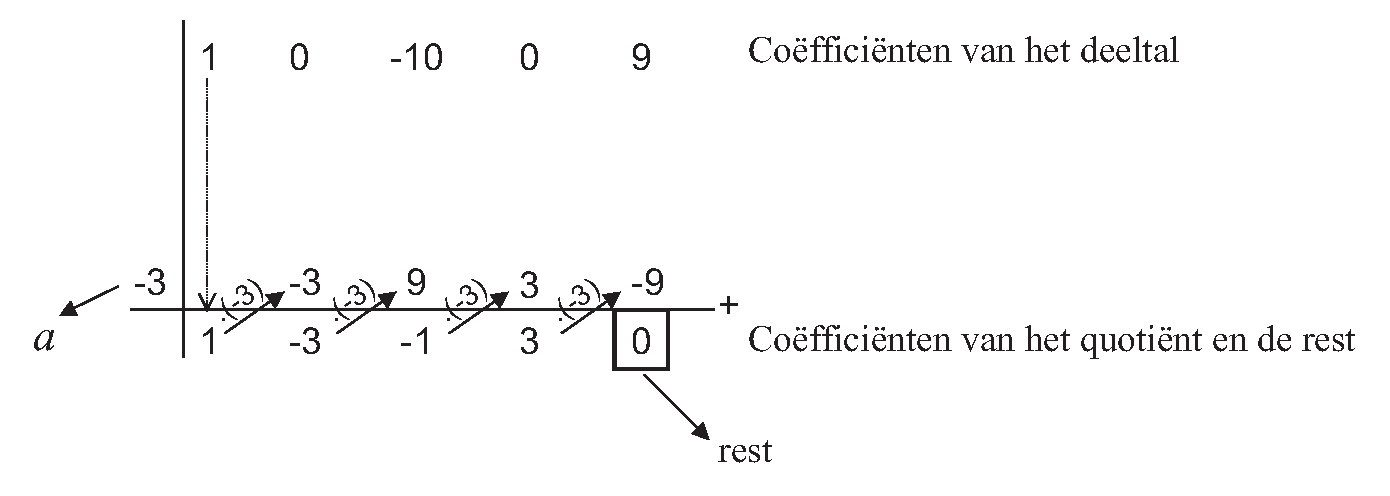
\includegraphics[height=4cm]{Horner}
\end{center}

\noindent Het quoti\"{e}nt is dus $x^3-3x^2-x+3$ en de rest is
$0$.

Hernemen we het voorbeeld uit Paragraaf~\ref{M01_euclidische deling},
nl.~de deling van $2x^3+x^2-5x+2$ door $x-3$. Daar hebben we deze
deling uitgevoerd m.b.v.~een deelschema. We maken nu deze deling
opnieuw d.m.v.~het rekenschema van Horner.

\begin{center}%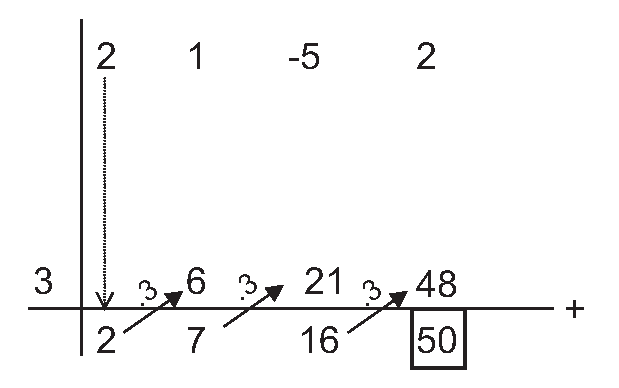
\includegraphics[height=3cm]{Horner2}
\end{center}

\noindent Merk op dat de rest $50$ ook de getalwaarde van het
deeltal voorstelt voor $x=3$, d.i.\[2\cdot3^3+3^2-5\cdot3+2=50.\]

\subsubsection*{Besluit}
\noindent\fbox{\parbox{\textwidth}{

\vspace{1.5ex}

Om de eventuele delers  van de vorm $x-a$ ($a \in \R$) van een
veelterm te vinden en het bijhorende quoti\"{e}nt te zoeken, ga je als volgt te werk:\\
\begin{enumerate}
\item Bepaal de delers van de constante term van de veelterm.
\item Bepaal de getalwaarde van de veelterm voor deze delers.
\item Als deze getalwaarde $0$ is, dan heeft de deling door $x-a$ (met $a$ deler van de constante term) rest $0$.
\item Bepaal dan het quoti\"{e}nt van de deling door een Euclidische deling uit te voeren of door het rekenschema van Horner toe te passen.
\end{enumerate}

\vspace{0.5ex}

}}

\noindent$\hookrightarrow$ \textit{Maak nu Oefening 4 van
Paragraaf~\ref{M01_oef}}.
\end{document}
